\chapter{Derivation of the Circle of Confusion}
\label{Appendix: CoC derivation}

The Circle of Confusion estimates through classical optical theory the amount of blur present in the image of an out of focus object, as explained by Greenleaf \cite{Greenleaf1950}. As shown in Figure \ref{fig: CoC geometry}, an object $O$ at a distance $d_f$ of a converging lens, with focal length $f$ and aperture $D$, produces an image $I$ at a distance $Z$ of this lens, as per the ideal lens equation. If an object $O'$ finds itself behind of $O$ by a defocus distance $l$, its image will form at $Z'$ on the opposite side of the converging lens. However, a point in object $O'$ will appear smeared into a circle in the plane of image $I$, as it is out of focus. To calculate the size of this circle, classic optics and geometry can be used.

\begin{figure}[htbp]
    \centering
    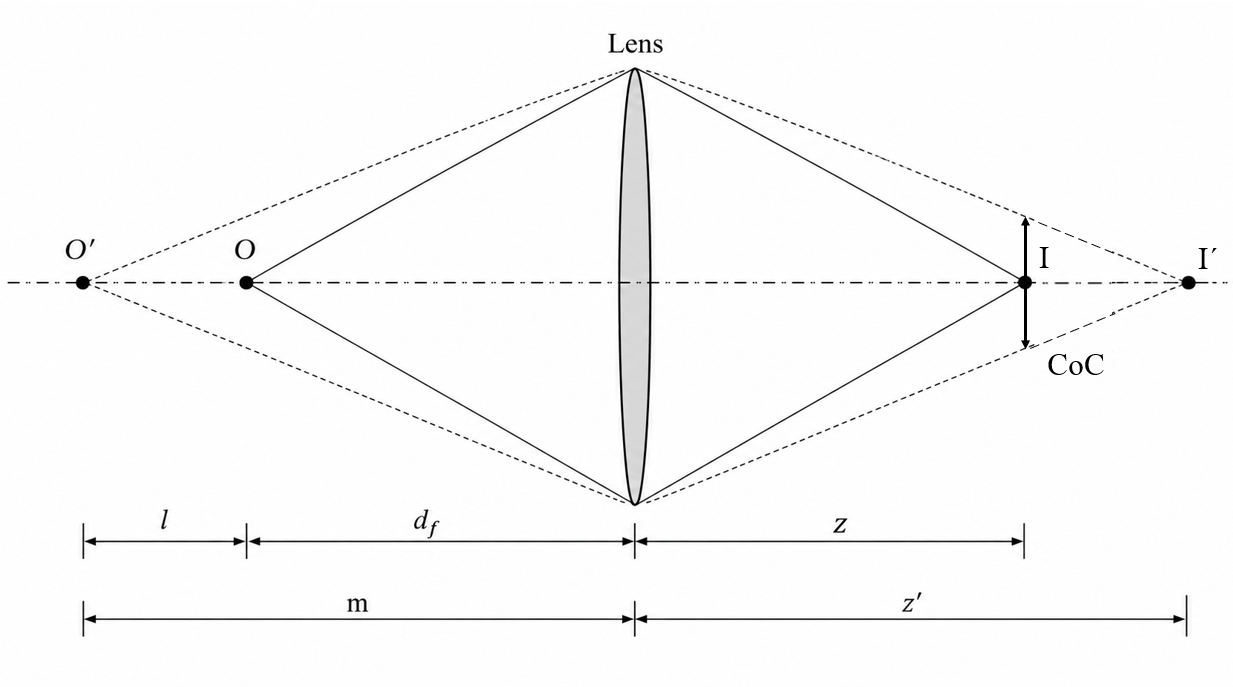
\includegraphics[width=0.8\textwidth]{figures/CoC drawing.png}
    \caption{Geometry of an out of focus object used to derive the CoC}
    \label{fig: CoC geometry}
\end{figure}

Through the ideal lens equation, $Z$ and $Z'$ can be written in the following form:


\begin{align}
    \label{equation: Z and Zprime}
    &Z = \frac{fd_f}{d_f-f}   & Z' = \frac{fm}{m - f}
\end{align}

Using triangle similarity, the relationship below can be established:

\begin{equation}
    \label{equation: CoC triangle similarity}
    \frac{CoC}{Z' - Z} = \frac{D}{Z'}
\end{equation}

Substituting Eq. \ref{equation: Z and Zprime} in relationship \ref{equation: CoC triangle similarity} and doing the necessary simplification, an explicit equation for $CoC$ is obtained:

\begin{equation}
    \label{equation: CoC explicit}
    CoC = \frac{f^2l}{f_\#m(d_f-f)}
\end{equation}

Where $f_\# = \frac{f}{D}$ is the lens f-stop number.

\par In Chapter \ref{chapter: methodology}, the sign of $l$ was considered to change depending on its position relative to the in-focus plane. This way, if an object finds itself behind the in-focus plane, Eq. \ref{equation: CoC explicit} will result in a negative $CoC$, while if the object is in front, it will be positive. Since the circle of confusion is a length, its absolute value can be considered in these cases.

\par Equation \ref{equation: CoC explicit} can also be modified by substituting it with Eq. \ref{equation: M and S definitions}, which define the magnification $Mag$ and sensitivity $S$

\begin{align}
        \label{equation: M and S definitions}
        &Mag = \frac{f}{d_f-f} & S = lMag
\end{align}

Resulting in:

\begin{align}
    \label{equation: CoC in M and S}
    & CoC = \frac{flMag}{f_\#m} & CoC = \frac{fS}{f_\#m}
\end{align}

The CoC is also in the core of another important parameter in optics called depth of field (DoF) \cite{Greenleaf1950}. The depth of field is the region around the in-focus plane where the $CoC$ is below a threshold deemed acceptable. This way, the depth of field can be interpreted as the thickness of the in-focus plane, where the image of all the objects inside this region is considered sharp enough. By definition, DoF can be calculated by subtracting the object distances $m_+$ and $m_-$ that produces the same $CoC$ when in front of the in-focus plane and behind it, respectively.
